\section{一次函数与二次函数}

\subsection{一次函数}

\begin{definition}
    一次函数是指形如 $f(x) = ax + b$ 的函数，其中 $a, b$ 为常数，且 $a \neq 0$。一次函数的图像是一条直线。
\end{definition}
\begin{definition}
    \begin{minipage}[c]{0.55\textwidth}
        $k=\frac{y_1-y_2}{x_1-x_2}$，$(x_1,y_1),(x_2,y_2)$为直线上两个不同的点

        只需要联立即可解：
        $$
            \begin{cases}
                y_1 = k x_1 + b \\
                y_2 = k x_2 + b
            \end{cases}
        $$
        这个式子还可以写为：

        $k=\tan \alpha,\alpha$为直线与$x$轴正半轴的夹角。
    \end{minipage}%
    \begin{minipage}[c]{0.45\textwidth}
        \centering
        \begin{tikzpicture}[scale=0.5, every node/.style={scale=0.8}]
            % 坐标轴
            \draw[->, thick] (-1,0) -- (5,0) node[below] {$x$};
            \draw[->, thick] (0,-1) -- (0,5) node[left] {$y$};
            \node[below left] at (0,0) {$O$};

            % 直线
            \draw[blue, thick, name path=line] (-0.5, 1) -- (4.5, 4) node[right] {$y=kx+b$};

            % 两个点
            \coordinate (P1) at (0.9, 1.78);
            \coordinate (P2) at (3, 3.18);
            \fill[red] (P1) circle (2pt) node[left] {$P_1(x_1, y_1)$};
            \fill[red] (P2) circle (2pt) node[above left] {$P_2(x_2, y_2)$};

            % 构造直角三角形
            \coordinate (P3) at (3, 1.75);
            \draw[dashed, red] (P1) -- (P3) -- (P2);

            % 标记斜率
            \node[red, below] at ($(P1)!0.5!(P3)$) {$x_2-x_1$};
            \node[red, right] at ($(P2)!0.5!(P3)$) {$y_2-y_1$};

            % 标记夹角
            \coordinate (inter) at (-2.5,0); % 直线与x轴交点
            \coordinate (p_on_x) at (0,0);
            \draw[->, orange] (1.6,1.78) arc (0:40:0.5) node[midway, right] {$\alpha$};
        \end{tikzpicture}
    \end{minipage}
\end{definition}
\begin{theorem}[截距]
    \begin{minipage}[c]{0.55\textwidth}
        一次函数的图像与 $x$ 轴的交点为 $(-\frac{b}{a}, 0)$，与 $y$ 轴的交点为 $(0, b)$。
    \end{minipage}%
    \begin{minipage}[c]{0.45\textwidth}
        \centering
        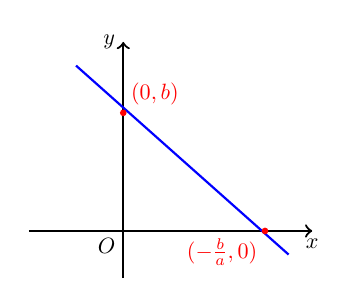
\begin{tikzpicture}[scale=0.6, every node/.style={scale=0.8}]
            % 坐标轴
            \draw[->, thick] (-2,0) -- (4,0) node[below] {$x$};
            \draw[->, thick] (0,-1) -- (0,4) node[left] {$y$};
            \node[below left] at (0,0) {$O$};

            % 直线
            \draw[blue, thick] (-1, 3.5) -- (3.5, -0.5);

            % 截距点
            \fill[red] (3,0) circle (2pt) node[below left] {$(-\frac{b}{a}, 0)$};
            \fill[red] (0,2.5) circle (2pt) node[above right] {$(0, b)$};
        \end{tikzpicture}
    \end{minipage}
\end{theorem}

\begin{example}
    求函数 $f(x) = 2x + 3$ 在 $x$ 轴上的截距和在 $y$ 轴上的截距。
\end{example}

\v{4em}

\begin{warning}
    截距也有正负之分！
\end{warning}

\begin{example}
    求直线 $y= 3x - 4$ 在 $x$ 轴和 $y$ 轴上的截距。
\end{example}

\v{4em}

\subsubsection{正比例函数}

\begin{definition}[正比例函数]
    形如$y=kx+b(k\ne 0)$的函数为一次函数。（$b=0$时为正比例函数，正比例函数也是一次函数）。
\end{definition}

\subsubsection{直线走势与斜率的关系}

\begin{theorem}
    \begin{minipage}[c]{0.55\textwidth}
        \begin{enumerate}
            \item $|k|$越大，直线越陡峭，越接近$y$轴；
            \item $|k|$越小，直线越平缓，越接近$x$轴。
            \item $k>0$，$y$随着$x$增大而增大；$k<0$，$y$随着$x$增大而减小。
        \end{enumerate}
    \end{minipage}%
    \begin{minipage}[c]{0.45\textwidth}
        \centering
        \begin{tikzpicture}[scale=0.4, every node/.style={scale=0.8}]
            % 坐标轴
            \draw[->, thick] (-3,0) -- (3,0) node[below] {$x$};
            \draw[->, thick] (0,-3) -- (0,3) node[left] {$y$};
            \node[below left] at (0,0) {$O$};

            % 不同斜率的直线
            \draw[blue, thick] (-2.5, -2.5*0.5) -- (2.5, 2.5*0.5) node[right] {$|k|$较小};
            \draw[red, thick] (-2, -2*1.2) -- (2, 2*1.2) node[right] {$|k|$较大};
            \draw[green!60!black, thick] (-2.5, 2.5) -- (2.5, -2.5) node[right] {$k<0$};
        \end{tikzpicture}
    \end{minipage}
\end{theorem}

\subsubsection{直线的单调性}
\begin{theorem}
    \begin{minipage}[c]{0.55\textwidth}
        若$x$取值范围为$x_1<x<x_2$ \\
        $k>0$时，$f(x_1)$为最小值，$f(x_2)$为最大值。 \\
        $k<0$时，$f(x_1)$为最大值，$f(x_2)$为最小值。
    \end{minipage}%
    \begin{minipage}[c]{0.45\textwidth}
        \centering
        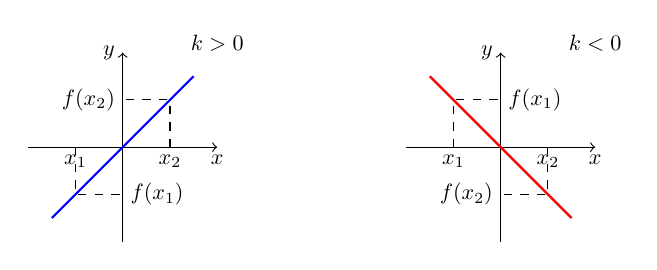
\begin{tikzpicture}[scale=0.6, every node/.style={scale=0.8}]
            % k>0
            \begin{scope}[xshift=-4cm]
                \draw[->] (-2,0) -- (2,0) node[below]{$x$};
                \draw[->] (0,-2) -- (0,2) node[left]{$y$};
                \draw[blue, thick] (-1.5,-1.5) -- (1.5,1.5);
                \draw[dashed] (-1,0) node[below]{$x_1$} -- (-1,-1) -- (0,-1) node[right]{$f(x_1)$};
                \draw[dashed] (1,0) node[below]{$x_2$} -- (1,1) -- (0,1) node[left]{$f(x_2)$};
                \node at (2,2.2) {$k>0$};
            \end{scope}
            % k<0
            \begin{scope}[xshift=4cm]
                \draw[->] (-2,0) -- (2,0) node[below]{$x$};
                \draw[->] (0,-2) -- (0,2) node[left]{$y$};
                \draw[red, thick] (-1.5,1.5) -- (1.5,-1.5);
                \draw[dashed] (-1,0) node[below]{$x_1$} -- (-1,1) -- (0,1) node[right]{$f(x_1)$};
                \draw[dashed] (1,0) node[below]{$x_2$} -- (1,-1) -- (0,-1) node[left]{$f(x_2)$};
                \node at (2,2.2) {$k<0$};
            \end{scope}
        \end{tikzpicture}
    \end{minipage}
\end{theorem}

\begin{example}[线性换元]
    若 $x \in [\frac{\pi}{3}, \frac{\pi}{4}]$，求：
    \begin{enumerate}
        \item $2x+\frac{\pi}{3}$ 的取值范围
        \item $-2x-\frac{\pi}{4}$ 的取值范围
    \end{enumerate}
\end{example}

\v{4em}

\subsubsection{直线的推论}

\begin{corollary}
    \begin{multicols}{2}
        \begin{itemize}
            \item $k=1$时，直线与$x$轴正半轴夹角为$45^\circ$
            \item $k=-1$时，直线与$x$轴正半轴夹角为$135^\circ$
            \item $k=\frac{\sqrt3}{3}$时，直线与$x$轴正半轴夹角为$30^\circ$
                  \columnbreak
            \item $k=-\frac{\sqrt3}{3}$时，直线与$x$轴正半轴夹角为$150^\circ$
            \item $k=\sqrt3$时，直线与$x$轴正半轴夹角为$60^\circ$
            \item $k=-\sqrt3$时，直线与$x$轴正半轴夹角为$120^\circ$
        \end{itemize}
    \end{multicols}
\end{corollary}

\begin{corollary}
    $k=0\Leftrightarrow$直线垂直于$y$轴。$k\to \infty$ 不存在$\Leftrightarrow$直线垂直于$x$轴。
\end{corollary}

\subsubsection{一次函数所过的象限问题}

\begin{table}[ht]
    \centering
    \caption{一次函数过的象限}
    \begin{tabular}{l|l|l}
              & $b>0$ & $b<0$ \\
        \hline
        $k>0$ & 一三二   & 一三四   \\
        \hline
        $k<0$ & 二四一   & 二四三   \\
        \hline
    \end{tabular}
\end{table}

\begin{example}
    一次函数$y=kx+b$在定义域$0\le x \le 2$内的最大值为$4$，最小值为$−2$，求一次函数的解析式。
\end{example}

\v{4em}

\begin{example}
    直线$y=kx+b$不经过第二象限，求$k$和$b$的取值范围。
\end{example}

\v{6em}

\pagebreak

\subsection{平移与对称}
\begin{theorem}
    \begin{minipage}[c]{0.55\textwidth}
        将一次函数$y=kx+b$沿着某个方向平移$a(a>0)$个单位。 \\
        向上平移后的解析式为$y=kx+b+a$ \\
        向下平移后的解析式为$y=kx+b-a$ \\
        向左平移后的解析式为$y=k(x+a)+b$ \\ % 修正为标准形式
        向右平移后的解析式为$y=k(x-a)+b$ \\ % 修正为标准形式
        口诀：左加右减，上加下减。
    \end{minipage}%
    \begin{minipage}[c]{0.45\textwidth}
        \centering
        \begin{tikzpicture}[scale=0.5, every node/.style={scale=0.8}]
            % 坐标轴
            \draw[->, thick] (-4,0) -- (4,0) node[below] {$x$};
            \draw[->, thick] (0,-3) -- (0,4) node[left] {$y$};

            % 原始直线
            \draw[gray, thick, dashed] (-3,-1) -- (3,2) node[right, black] {$y=kx+b$};

            % 上下平移
            \draw[blue, thick] (-3,0.5) -- (3,3.5);
            \draw[->, blue] (0,1) -- (0,2.5) node[midway, right] {上移};

            % 左右平移
            \draw[red, thick] (-1,-1) -- (5,2);
            \draw[->, red] (1,1) -- (2.5,1) node[midway, above] {右移};
        \end{tikzpicture}
    \end{minipage}
\end{theorem}
\begin{theorem}
    \begin{minipage}[c]{0.55\textwidth}
        将一次函数$y=kx+b$沿着某个方向作对称变换。\\
        沿着$x$轴对称后的解析式为$y=-kx-b$ \\
        沿着$y$轴对称后的解析式为$y=-kx+b$ \\
        关于原点对称后的解析式为$y=kx-b$ % 注意：原文这里有误，应为-y=k(-x)+b => y=-kx-b。但关于原点对称是y=-f(-x) => y=-k(-x)+b = kx-b，此处以y=f(x)关于原点对称是y=-f(-x)为准则。
    \end{minipage}%
    \begin{minipage}[c]{0.45\textwidth}
        \centering
        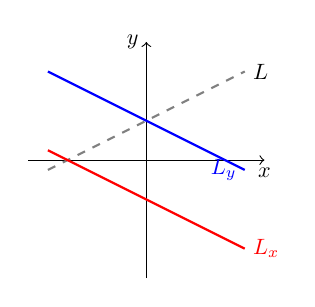
\begin{tikzpicture}[scale=0.5, every node/.style={scale=0.8}]
            \draw[->] (-3,0) -- (3,0) node[below] {$x$};
            \draw[->] (0,-3) -- (0,3) node[left] {$y$};

            % 原始直线
            \draw[gray, thick, dashed] (-2.5, -0.25) -- (2.5, 2.25) node[right, black] {$L$};

            % 关于y轴对称
            \draw[blue, thick] (-2.5, 2.25) -- (2.5, -0.25) node[left, blue] {$L_y$};

            % 关于x轴对称
            \draw[red, thick] (-2.5, 0.25) -- (2.5, -2.25) node[right, red] {$L_x$};
        \end{tikzpicture}
    \end{minipage}
\end{theorem}

\begin{warning}
    对于所有的函数和方程，在图像上的平移都只针对 $x$ 或 $y$ 而言。

    例如 $\sin (3x+\frac{\pi}{6})$ 如果向左平移 $\frac6\pi$ 个单位长度呢？
\end{warning}

\begin{example}
    点$C$为直线$y=x$上与原点不重合的点，直线$y=2x+1$与$x$轴和$y$轴分别交于$A,B$两点，
    将直线沿着射线$OC$方向平移$3\sqrt2$个单位，求平移后直线的解析式。
\end{example}

\v{10em}

\begin{example}
    将一次函数$y=-3x+4$向下平移$1$个单位相当于向\underline{\quad}(填左或右)平移\underline{\quad}个单位。
\end{example}

\v{6em}

\subsection{垂直直线的斜率关系}
\begin{theorem}
    \begin{minipage}[c]{0.55\textwidth}
        若直线$y=k_1x+b_1$与直线$y=k_2x+b_2$相垂直，则有：$$k_1·k_2=-1$$
    \end{minipage}%
    \begin{minipage}[c]{0.45\textwidth}
        \centering
        \begin{tikzpicture}[scale=0.5, every node/.style={scale=0.8}]
            \draw[->] (-3,0) -- (3,0) node[below] {$x$};
            \draw[->] (0,-3) -- (0,3) node[left] {$y$};

            % 两条垂直直线
            \draw[blue, thick, name path=L1] (-2, -2) -- (2.5, 2.5) node[right] {$L_1$};
            \draw[red, thick, name path=L2] (-2, 2.5) -- (2, -1.5) node[right] {$L_2$};

            \node at (1.5, -2.5) {$k_1 \cdot k_2 = -1$};
        \end{tikzpicture}
    \end{minipage}
\end{theorem}

\begin{example}
    已知坐标系内两点$A(x_1,y_1),B(x_2,y_2)$，求线段$AB$垂直平分线的解析式。
\end{example}

\begin{solution}
    设线段$AB$垂直平分线的解析式为$y=kx+b$，则有：
    $$\begin{cases}k·\frac{y_1-y_2}{x_1-x_2}=-1 \\ \frac{y_1+y_2}{2}=k·\frac{x_1+x_2}{2}+b \\ \end{cases}$$
\end{solution}

\begin{corollary}
    点$(a,b)$关于直线$y=x$的对称点为$(b,a)$ \\
    点$(a,b)$关于直线$y=-x$的对称点为$(-b,-a)$
\end{corollary}

\begin{example}
    在平面直角坐标系中，定义点$(-b,-a)$为点$(a,b)$的关联点。若一个点和它的关联点在同一个象限，判断该点所在的象限。
\end{example}

\v{6em}

\begin{example}
    在平面直角坐标系中，$A(0,3),B(4,0)$，点$C$在坐标轴上且满足$CA=CB$，求$C$点坐标。
\end{example}

\v{6em}

\begin{example}
    若直线$y_1=3x+2$与直线$y_2=kx+b$关于直线$y=x$对称，求直线$y_2$的解析式。
\end{example}

\v{6em}

\subsection{直线交点与方程解的关系}
\begin{theorem}
    \begin{minipage}[c]{0.5\textwidth}
        已知直线$y=k_1x+b_1$和直线$y=k_2x+b_2$ \\
        若$k_1\ne k_2$，两条直线有唯一交点。 \\
        若$k_1 = k_2, b_1 \ne b_2$，两条直线平行，没有交点。 \\
        若$k_1 = k_2, b_1 = b_2$，两条直线重合，有无数个交点。
    \end{minipage}%
    \begin{minipage}[c]{0.45\textwidth}
        \centering
        \begin{tikzpicture}[scale=0.6, every node/.style={scale=0.8}]
            % 相交
            \draw[blue] (-2,-1) -- (2,3);
            \draw[red] (-2,3) -- (2,1);
            \node at (0,-1.5) {相交};

            % 平行
            \begin{scope}[xshift=4cm]
                \draw[blue] (-1,-1) -- (1,3);
                \draw[red] (-1.5,-1) -- (0.5,3);
                \node at (0,-1.5) {平行};
            \end{scope}

            % 重合
            \begin{scope}[xshift=8cm]
                \draw[blue, line width=2pt] (-1,-1) -- (1,3);
                \draw[red, dashed, line width=0.5pt] (-1,-1) -- (1,3);
                \node at (0,-1.5) {重合};
            \end{scope}
        \end{tikzpicture}
    \end{minipage}
\end{theorem}

\begin{theorem}
    \begin{minipage}[c]{0.4\textwidth}
        直线$y=k_1x+b_1$与直线$y=k_2x+b_2$的交点$(x_0,y_0)$是方程组 \\
        $$\begin{cases} k_1x-y+b_1=0  \\ k_2x-y+b_2=0  \\ \end{cases}$$
        的解。
        \begin{center}
            \begin{itemize}
                \item 两条直线有唯一交点 $\Leftrightarrow$ 方程组有唯一解。
                \item 两条直线平行 $\Leftrightarrow$ 方程组无解。
                \item 两条直线重合 $\Leftrightarrow$ 方程组有无数解。
            \end{itemize}
        \end{center}
    \end{minipage}%
    \begin{minipage}[c]{0.55\textwidth}
        \centering
        \begin{tikzpicture}[scale=0.7, every node/.style={scale=0.8}]
            \draw[->, thick] (-1,0) -- (4,0) node[below] {$x$};
            \draw[->, thick] (0,-1) -- (0,4) node[left] {$y$};

            % 直线
            \draw[blue, thick] (-0.5, 0) -- (3.5, 4);
            \draw[red, thick] (-0.4, 4) -- (3.5, 0);

            % 交点
            \coordinate (inter) at (1.5, 2);
            \fill[black] (inter) circle (2pt) node[above right] {交点 $(x_0, y_0)$};
            \draw[dashed] (inter) -- (1.5,0) node[below] {$x_0$};
            \draw[dashed] (inter) -- (0,2) node[left] {$y_0$};
        \end{tikzpicture}
    \end{minipage}
\end{theorem}

\begin{example}
    设$b>a$，在同一直角坐标系下画出一次函数$y=bx+a$和一次函数$y=ax+b$的图像。
\end{example}

\v{6em}

\begin{example}
    直线$y=3x-1$与直线$y=x-k$的交点在第四象限，求$k$的取值范围。
\end{example}

\v{6em}

\subsection{一次函数与不等式}
\begin{theorem}
    \begin{minipage}[c]{0.65\textwidth}
        若一次函数$y=kx+b$与$x$轴交点为$(x_0,0)$，则有： \\
        方程$kx+b=0$的解为$x=x_0$.
        \begin{itemize}
            \item 若$k>0$，不等式$kx+b>0$的解集为$x>x_0$
            \item 若$k<0$，不等式$kx+b>0$的解集为$x<x_0$
        \end{itemize}
    \end{minipage}%
    \begin{minipage}[c]{0.3\textwidth}
        \centering
        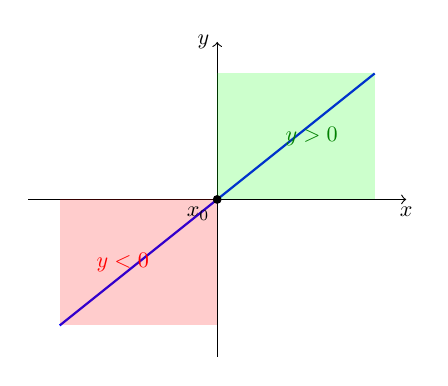
\begin{tikzpicture}[scale=0.8, every node/.style={scale=0.8}]
            \draw[->] (-3,0) -- (3,0) node[below] {$x$};
            \draw[->] (0,-2.5) -- (0,2.5) node[left] {$y$};

            % k>0
            \draw[blue, thick] (-2.5,-2) -- (2.5,2);
            \fill[green, opacity=0.2] (0,0) rectangle (2.5,2);
            \fill[red, opacity=0.2] (-2.5,-2) rectangle (0,0);

            \node[green!50!black] at (1.5, 1) {$y>0$};
            \node[red] at (-1.5, -1) {$y<0$};

            \fill (0,0) circle (2pt) node[below left] {$x_0$};
        \end{tikzpicture}
    \end{minipage}
\end{theorem}
\begin{theorem}
    \begin{minipage}[c]{0.55\textwidth}
        若一次函数$y=k_1x+b_1$与一次函数$y=k_2x+b_2$相交于$(x_0,y_0)$，且$k_1>k_2$，则有：
        \begin{itemize}
            \item  $k_1x+b_1>k_2x+b_2$的解集为$x>x_0$
            \item $k_1x+b_1<k_2x+b_2$的解集为$x<x_0$
        \end{itemize}
    \end{minipage}%
    \begin{minipage}[c]{0.45\textwidth}
        \centering
        \begin{tikzpicture}[scale=0.6, every node/.style={scale=0.8}]
            \draw[->] (-3,0) -- (3,0) node[below] {$x$};
            \draw[->] (0,-3) -- (0,3) node[left] {$y$};

            \draw[blue, thick, name path=L1] (-2,-2.5) -- (2.5,2.5) node[right] {$y_1$};
            \draw[red, thick, name path=L2] (-2.5,2) -- (2,0) node[right] {$y_2$};

            \path [name intersections={of=L1 and L2, by={i}}];
            \draw[dashed] (i) -- (i |- 0,0) node[below] {$x_0$};

            \node at (2,-1) {$x>x_0 \implies y_1>y_2$};
            \node at (-1.5,2) {$x<x_0 \implies y_1<y_2$};
        \end{tikzpicture}
    \end{minipage}
\end{theorem}

\begin{theorem}
    \begin{minipage}[c]{0.55\textwidth}
        如下图，若一次函数$y=k_1x+b_1$反比例函数$y=\frac{k_2}{x}$两支相交于$N(x_1,y_1),M(x_2,y_2)$两点，则有：
        \begin{itemize}
            \item         $k_1x+b_1>\frac{k_2}{x} \Leftrightarrow x_1<x<0$或$x>x_2$
            \item           $k_1x+b_1<\frac{k_2}{x} \Leftrightarrow x<x_1$或$0<x<x_2$
        \end{itemize}
    \end{minipage}%
    \begin{minipage}[c]{0.45\textwidth}
        \centering
        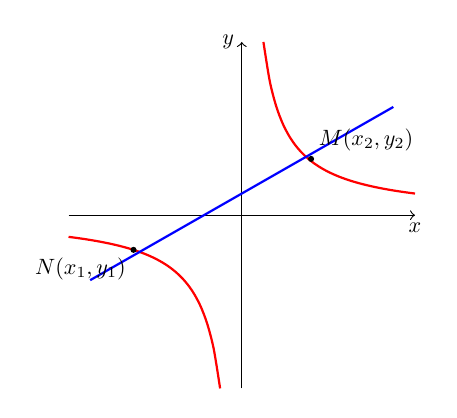
\begin{tikzpicture}[scale=0.55, every node/.style={scale=0.8}]
            \draw[->] (-4,0) -- (4,0) node[below] {$x$};
            \draw[->] (0,-4) -- (0,4) node[left] {$y$};

            % 反比例函数
            \draw[red, thick] plot[smooth, domain=0.5:4] (\x, {2/\x});
            \draw[red, thick] plot[smooth, domain=-4:-0.5] (\x, {2/\x});

            % 一次函数
            \draw[blue, thick] (-3.5,-1.5) -- (3.5, 2.5);

            % 交点
            \fill (-2.5,-0.8) circle (2pt) node[below left] {$N(x_1,y_1)$};
            \fill (1.6,1.3) circle (2pt) node[above right] {$M(x_2,y_2)$};
        \end{tikzpicture}
    \end{minipage}
\end{theorem}

\begin{example}
    一次函数$y=kx+b$与$x$轴交于$(2,0)$，求不等式$kx+b>3k$的解集。
\end{example}

\v{6em}

\begin{example}
    一次函数$y=k_1x+b_1$和一次函数$y_2=k_2x+b_2$满足无论$x$取何值，$y_1>y_2$恒成立，判断$k_1$与$k_2$，$b_1$与$b_2$的关系。
\end{example}

\v{6em}

\begin{example}
    一次函数$y_1=3x+2$和一次函数$y_2=\frac{1}{3}x-\frac{2}{3}$满足$x>m$时，$y_1>y_2$恒成立，求$m$的取值范围。
\end{example}

\v{6em}

\begin{example}
    已知$f(x)=x-1,g(x)=\frac{2}{x}$，定义$h(x)=\max(f(x),g(x))$，
    其中$\max(a,b)=
        \begin{cases}
            a & \text{$a \ge b$}
            \\ b & \text {$a<b$}
        \end{cases}$，即取两者的最大值。
    求$h(x)$的最小值。
\end{example}

\v{6em}

\subsection{一次函数中的坐标轴问题}

\begin{example}
    直线$y=kx+5$与坐标轴围成的三角形的周长为30，求$k$的值。
\end{example}

\v{8em}

\begin{example}
    直线$y=kx-3$与坐标轴围成的三角形的面积为6，求$k$的值。
\end{example}

\v{8em}

\begin{example}
    直线$y=kx+b$图像经过点$P(3,2)$且与$x$轴正半轴和$y$轴正半轴分别交于$A,B$两点，且$OA+OB=12$，求一次函数的解析式。
\end{example}

\v{8em}

\subsection{一次函数中的面积问题}

\begin{theorem}
    \begin{minipage}[c]{0.55\textwidth}
        如图，$\triangle ABC$面积可以表示为$\frac{1}{2}$水平宽·铅垂高。

        设$A(x_1,y_1),B(x_2,y_2),C(x_3,y_3)$

        根据$A,B$坐标算出直线的解析式，求出$D$点坐标$(x_4,y_4)$：
        $$
            S_{\triangle ABC}=\frac{1}{2}|x_2-x_1||y_3-y_4|
        $$
    \end{minipage}%
    \begin{minipage}[c]{0.45\textwidth}
        \begin{tikzpicture}[scale=0.5,
                every node/.style={scale=1.0}, % 统一放大节点文字
                axis/.style={->, thick}, % 坐标轴样式
                line/.style={thick}, % 普通线条样式
                dashed line/.style={thick, dashed} % 虚线样式
            ]
            \draw[axis] (-0.5, 0) -- (7, 0) node[below] {$x$};
            \draw[axis] (0, -0.5) -- (0, 6) node[left] {$y$};
            \node[below left] at (0,0) {$O$};

            \coordinate (A) at (1.5, 1);
            \coordinate (B) at (5.5, 2.5);
            \coordinate (C) at (4, 5);

            \draw[line] (A) -- (B) -- (C) -- cycle;

            \coordinate (H) at (B |- A);
            \draw[dashed line, red] (A) -- (H);
            \draw[dashed line] (B) -- (H);

            \coordinate (D) at (4,1.9);
            \draw[dashed line, green!50!black] (C) -- (D);

            \node[below left] at (A) {$A$};
            \node[above right] at (B) {$B$};
            \node[above] at (C) {$C$};
            \node[below left=2pt] at (D) {$D$};

            \node[align=center] at ($(C)!0.5!(D)$)[right=5pt] {铅垂高};
            \node at ($(A)!0.5!(H)$)[below=1pt] {水平宽};
        \end{tikzpicture}
    \end{minipage}
\end{theorem}

\subsection{一次函数过定点问题}

\begin{example}
    求一次函数$y=(2-k)x+3k$过的定点。
\end{example}

\begin{solution}
    一次函数过定点，说明存在一组点$(x,y)$满足无论$k$取何值，等式$y=(2-k)x+3k$恒成立。
    说明$k$的所有系数为零。

    根据：
    $(3-x)k+2x-y=0$
    可得：
    $$\begin{cases}
            3-x=0  \\
            2x-y=0 \\
        \end{cases} \Rightarrow x=3,y=6$$
    所以一次函数过定点(3,6)
\end{solution}

\v{2em}

\begin{example}
    若$(2k-1)x-(k-3)y-(k-4)=0$是$y$关于$x$的一次函数，求$k$的取值范围，并求出当$k$满足取值范围时，一次函数恒过的定点。
\end{example}

\v{6em}

\begin{example}
    平面直角坐标系有两点$A(4,5),B(6,9)$，若一次函数$y=kx-2k+3$与线段$AB$有交点，求$k$的取值范围。
\end{example}

\v{6em}

\subsection{一次函数与将军饮马问题}

\begin{theorem}
    如图，在直线$l$上找一点$P$，使得以下结论成立.
    \begin{enumerate}
        \item $PB+PA$最小，作$B$关于$l$的对称点$B'$，$P$为$AB'$与$l$的交点。最小值为$|AB'|$
        \item $|PA-PB|$最小，$P$为线段$AB$垂直平分线与$l$的交点。最小值为0
        \item $|PA-PB|$最大，$P$为$AB$延长线与$l$的交点。最大值为$|AB|$
    \end{enumerate}

    \begin{center}
        \begin{tikzpicture}
            \coordinate (A) at (3, 1.5);
            \coordinate (B) at (1.5, 1);
            \draw (0,0) -- (5,0);
            \node[left=3pt] at (0,0) {$l$};
            \fill (A) circle (1.5pt);
            \node[above=2pt] at (A) {A};
            \fill (B) circle (1.5pt);
            \node[above=2pt] at (B) {B};
        \end{tikzpicture}
    \end{center}
\end{theorem}

\begin{example}
    已知平面直角坐标系两点$A(2,3),B(4,5)$，$C$在$x$轴上，求满足下列条件的$C$的坐标以及相应的最值。
    \begin{itemize}
        \item $CA+CB$最小
        \item $|CA-CB|$最小
        \item $|CA-CB|$最大
    \end{itemize}
\end{example}

\v{10em}

\subsection{两点之间的距离构造}

\begin{theorem}[两点间的距离公式]
    在平面直角坐标系中，已知两点$A(x_1,y_1),B(x_2,y_2)$，则有：
    \begin{itemize}
        \item $AB=\sqrt{(x_2-x_1)^2+(y_2-y_1)^2}$
    \end{itemize}
\end{theorem}

\begin{example}
    \begin{itemize}
        \item 求根式$\sqrt{x^2-4x+13}+\sqrt{x^2-8x+41}$的最小值，并求出取最小值时$x$的取值。
        \item 求根式$\sqrt{x^2-8x+41}-\sqrt{x^2-4x+13}$的最大值，并求出取最大值时$x$的取值。
    \end{itemize}
\end{example}

\v{10em}

\begin{example}
    已知平面直角坐标系两点$A(4,6),B(6,4)$，$C$在$y$轴上，$D$在$x$轴上，求使得四边形$ABCD$周长最小的$D$点坐标。
\end{example}

\v{10em}

\subsection{一次函数几何综合}

\begin{example}
    已知一次函数$y=-2x+4$的图像与$x$轴、$y$轴分别交于点$B,A$，以$AB$为边在第一象限内作等腰直角三角形$ABC$，且$\angle ABC=90^\circ$，
    $BA=BC$，作$OB$的垂直平分线$l$交直线$AB$于点$E$，交$x$轴于点$G$.
    \begin{enumerate}
        \item 求点$C$的坐标。
        \item 在$OB$垂直平分线$l$上有一点$M$，且点$M$与点$C$位于直线$AB$的同侧，使得$2S_{\triangle ABM}=S_{\triangle ABC}$,求点$M$的坐标。
        \item 在 (2) 的条件下，联结$CE,CM$, 判断$\triangle CEM$的形状，并给予证明。
    \end{enumerate}
\end{example}

\begin{figure}[H]
    \centering
    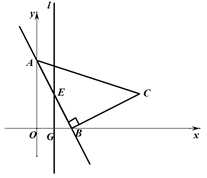
\includegraphics[width=4cm]{picture/401.png}
\end{figure}

\subsection{一次函数图像分析}

\begin{example}
    甲、乙两人在笔直的湖边公路上同起点、同终点、同方向匀速步行2400米，先到终点的人原地休息。
    已知甲先出发4分钟，在整个步行过程中，甲、乙两人间的距离（米）与甲出发的时间（分）之间的关系如图中折线
    $OA-AB-BC-CD$所示。
    \begin{itemize}
        \item 求线段$AB$的表达式，并写出自变量$x$的取值范围。
        \item 求乙的步行速度。
        \item 求点$C,D$的坐标。
    \end{itemize}
\end{example}

\begin{figure}[H]
    \centering
    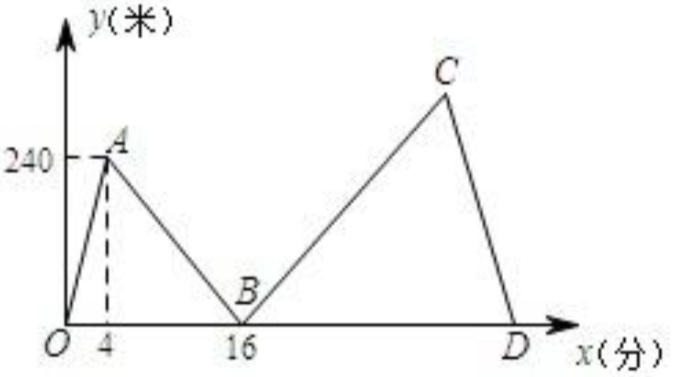
\includegraphics[width=6cm]{picture/6122.png}
    \caption{练习图}
\end{figure}

\subsection{一次函数与实际应用}

\begin{example}
    某自来水公司每月用水收费标准如下：每月固定水处理费$a$元，若当月用水量未超过$b$升，每升水价格为$c$元。
    若超过$b$升，超过的部分每升水的单价为$1.5c$元。已知当月有三户人家用水量与计价如下表所示，求$a,b,c$的值。
\end{example}
\begin{table}[ht]
    \centering
    \caption{用户用水量}
    \begin{tabular}{|l|l|l|}
        \hline
        用户 & 用水量(升) & 价格(元) \\
        \hline
        A  & 6      & 16    \\
        \hline
        B  & 8      & 20    \\
        \hline
        C  & 16     & 42    \\
        \hline
    \end{tabular}
\end{table}

\section{二次函数}

\begin{definition}
    二次函数是指形如 $f(x) = ax^2 + bx + c$ 的函数，其中 $a, b, c$ 为常数，且 $a \neq 0$。二次函数的图像是一条抛物线。
\end{definition}

\begin{theorem}[顶点]
    二次函数的顶点坐标为 $\left(-\frac{b}{2a}, f\left(-\frac{b}{2a}\right)\right)$，开口方向由 $a$ 的符号决定：$a > 0$ 时开口向上，$a < 0$ 时开口向下。
\end{theorem}

\subsubsection{求根公式与韦达定理}

\begin{theorem}[求根公式]
    二次方程 $ax^2 + bx + c = 0$ 的根为：
    $$
        x_{1,2} = \frac{-b \pm \sqrt{b^2 - 4ac}}{2a}
    $$
\end{theorem}

\begin{example}
    求方程 $2x^2 - 4x + 1 = 0$ 的根。
\end{example}

\v{4em}

\begin{theorem}[韦达定理]
    对于二次方程 $ax^2 + bx + c = 0$，设其根为 $x_1, x_2$，则有：
    \begin{align*}
        x_1 + x_2 & = -\frac{b}{a} \\
        x_1 x_2   & = \frac{c}{a}
    \end{align*}
\end{theorem}

\begin{warning}
    韦达定理使用的前提条件一定是方程具有两个根，即 $\triangle \geq 0$
\end{warning}

\begin{example}
    已知 $x_1$ 和 $x_2$ 为一元二次方程 $2 x^2-2 x+3 m-1=0$ 的两个实根，并 $x_1$ 和 $x_2$ 满足不等式 $\frac{x_1 x_2}{x_1+x_2-4}<1$ ，则实数 $m$ 取值范围是 \underline{\qquad}.
\end{example}

\v{8em}

\begin{example}
    已知关于 $x$ 的一元二次方程 $8 x^2+(m+1) x+m-7=0$ 有两个负数根，那么实数 $m$ 的取值范围是 \underline{\qquad}.
\end{example}

\v{8em}

\begin{theorem}[常用的韦达定理构造]
    \begin{multicols}{2}
        \begin{enumerate}
            \item $x_1^2+x_2^2=\left(x_1+x_2\right)^2-2 x_1 x_2$
            \item $\left(x_1-x_2\right)^2=\left(x_1+x_2\right)^2-4 x_1 x_2$
            \item $\frac{1}{x_1}+\frac{1}{x_2}=\frac{x_1+x_2}{x_1 x_2}$
            \item $\frac{x_2}{x_1}+\frac{x_1}{x_2}=\frac{x_1^2+x_2^2}{x_1 x_2}=\frac{\left(x_1+x_2\right)^2-2 x_1 x_2}{x_1 x_2}$
            \item $\frac{1}{x_1^2}+\frac{1}{x_2^2}=\frac{x_1^2+x_2^2}{x_1^2 x_2^2}=\frac{\left(x_1+x_2\right)^2-2 x_1 x_2}{x_1^2 x_2^2}$
            \item $x_1 x_2^2+x_1^2 x_2=x_1 x_2\left(x_1+x_2\right)$
                  \columnbreak
            \item $\left(x_1+m\right)\left(x_2+m\right)=x_1 x_2+m\left(x_1+x_2\right)+m^2$
            \item $x_1-x_2= \pm \sqrt{\left(x_1-x_2\right)^2}= \pm \sqrt{\left(x_1+x_2\right)^2-4 x_1 x_2}$
            \item $\left|x_1-x_2\right|=\sqrt{\left(x_1-x_2\right)^2}=\sqrt{\left(x_1+x_2\right)^2-4 x_1 x_2}$
            \item $\left|x_1\right|+\left|x_2\right|=\sqrt{\left(\left|x_1\right|+\left|x_2\right|^2\right)}=\sqrt{x_1^2+x_2^2+2\left|x_1\right|\left|x_2\right|}=\sqrt{\left(x_1+x_2\right)^2-2 x_1 x_2+2\left|x_1\right|\left|x_2\right|}$
        \end{enumerate}
    \end{multicols}
\end{theorem}

\begin{example}
    如果 $a$、$b$ 都是质数，且 $a^2-13 a+m=0, b^2-13 b+m=0$ ，那么 $\frac{b}{a}+\frac{a}{b}$ 的值为 （\qquad）
    \begin{tasks}(4)
        \task $\frac{123}{22}$
        \task $\frac{125}{22}$ 或 2
        \task $\frac{125}{22}$
        \task $\frac{123}{22}$ 或 2
    \end{tasks}
\end{example}

\v{6em}

\begin{example}
    设 $x_1$、$x_2$ 是方程 $2 x^2-4 m x+2 m^2+3 m-2=0$ 的两个实数根，当 m 为何值时，$x_1{ }^2+x_2{ }^2$有最小值？并求出这个最小值.
\end{example}

\v{6em}

\begin{example}
    已知 $\alpha$、$\beta$ 是方程 $x^2-x-1=0$ 的两个根，则 $\alpha^4+3 \beta$ 的值为 \underline{\qquad}.
\end{example}

\begin{solution}
    这里把 $\alpha$ 代入这个方程当中，可以得到 $\alpha^2=\alpha+1$，则 $\alpha^4$ 就出来了，再结合 $\alpha + \beta = 1$ 可以求出结果。
\end{solution}

\v{4em}

\begin{example}
    方程 $x^2+p x+1997=0$ 恰有两个正整数根 $x_1$、$x_2$ ，则 $\frac{p}{\left(x_1+1\right)\left(x_2+1\right)}$ 的值是 （\qquad）
    \begin{tasks}(4)
        \task 1
        \task -1
        \task $-\frac{1}{2}$
        \task $\frac{1}{2}$
    \end{tasks}
\end{example}

\v{6em}